\section{Building a Benchmark with Known Truth}
\label{sec:benchmark}

\subsection{What a benchmark needs}
\label{sec:benchmark-needs}

An injection test supplies the missing truth, since the true atmosphere of
WASP-17~b is unknown and real observations cannot show which pipeline
recovers the correct spectrum. A known transmission spectrum is written into
detector data, and each method's recovered spectrum is compared with the
injected one. To be useful, the comparison must meet four conditions.
Firstly, the injected truth must be known exactly. Secondly, the data should
be real wherever possible, so that the noise, detector flags, background and
field stars are those of an actual observation. Thirdly, every method must
start from the same injected raw data, infer its own transit geometry, and
see the truth only after its prediction is fixed. Finally, the comparison
must include a construction of the source independent of the assumption being
tested. Generating synthetic data with the same model later used to analyse
them is known as an inverse crime \citep{KaipioSomersalo2007}, and it can
hide the errors caused by a wrong model. The injectors I built during the first year to provide such a test failed, and what their failures taught me is set out in the rest of this section. The last of these lessons determines the design of the
benchmark in Section~\ref{sec:measured-benchmark}.

\subsection{Injecting into the raw data}
\label{sec:raw-injection}

The first lesson concerned where the transit is added. My first injector
added it to the calibrated integrations, after the pipeline's detector
stages. This was fast but bypassed the stages in which the methods differ in
their treatment of $1/f$ noise, saturated pixels and cosmic rays, and in
which \nova{}'s detector processing borrows steps from exoTEDRF
(Section~\ref{sec:nova}). I therefore moved the injection to the raw ramps,
and each method received its own native input product derived from the common
injected ramps. The new injector took the real pre-transit integrations of
WASP-17~b and removed, read by read, the light that the injected transit
would block.

\subsection{Which light belongs to the star}
\label{sec:which-light}

To remove this light, the injector needs a map of the starlight on the
detector, since the transit dims only the star. Close to the centre of each
trace the star dominates, and the map is well determined. Further out, in the
wings of the traces and in the faint light between them, part of the light
may come from the zodiacal background, other stars or the detector itself.
The WASP-17~b data alone cannot say how much. My first map, the lower
estimate, contained 0.9 to 5.0\% less light than observed in the extraction
box, treating the remainder as background. I bracketed this unresolved choice
with an upper estimate, in which all the light observed in the box is
starlight.

\begin{figure}[t]
  \centering
  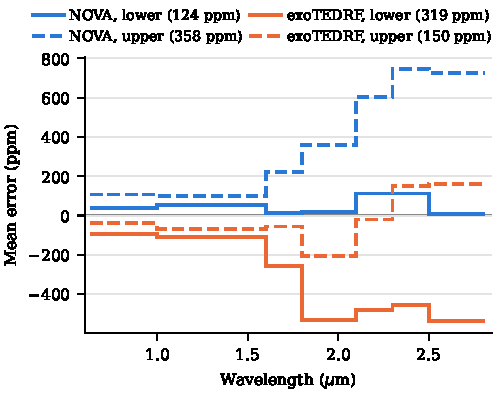
\includegraphics[width=\columnwidth]{figures/benchmark_flip_regional_errors.pdf}
  \caption{Mean error of the spectra recovered by \nova{} (blue) and exoTEDRF
  (orange) from the reference atmosphere injected into the WASP-17~b data, in
  seven wavelength regions, under the lower (solid) and upper (dashed)
  estimates of the starlight. The error is the recovered minus the injected
  depth, so a positive value means that the recovered transit is too deep. The
  legend gives the root-mean-square error over all 147 spectral bins in ppm.
  Both pipelines reduced raw data made with the same injection recipe, each
  with its own processing.}
  \label{fig:flip}
\end{figure}

Figure~\ref{fig:flip} shows the consequence of this choice for the reference
atmosphere. Under the lower estimate, \nova{} recovered the injected spectrum
with a root-mean-square error of 124~ppm and exoTEDRF with 319~ppm. Under the
upper estimate the order reversed, with 358~ppm for \nova{} and 150~ppm for
exoTEDRF.

The out-of-transit frames are identical in the two cases, and only the light
removed during the transit differs. Each pipeline measures the depth as the
light lost divided by its own estimate of the starlight, so both errors moved
in the same direction, by about 500~ppm in the red. The difference between
their mean errors barely changed, from 276 to 289~ppm. The injector's
assumption moved both pipelines together and decided which ended up closer to
the truth. The benchmark therefore rewarded the pipeline whose estimate of
the starlight agreed with the injector's, an agreement that the WASP-17~b
data could not check. The test showed that the ranking is sensitive to this
assumption for one atmosphere, but not which pipeline is right on the real
data.

The comparison also showed the danger of a shared model, which the fourth
condition guards against. \nova{}'s model of the starlight closely matches
the lower estimate, which treats about 2 to 4\% of the red light in the box
as background, so the lower-estimate benchmark risked favouring \nova{}
through this agreement. After its own background subtraction, exoTEDRF treats
all the remaining light in its box as starlight, and so matches the upper
estimate. Under the lower estimate, a grey transit, whose depth is the same at every wavelength, showed the resulting dilution directly, since exoTEDRF recovered only 0.969 of the injected depth in the red. Removing this dilution reduced
exoTEDRF's error from 319 to 116~ppm.

I also tested whether the real WASP-17~b data could settle the split between starlight and background. If all
the light in the extraction box is starlight, the transit dims the box by the
same fraction as the centre of the trace, and the ratio of the two dips is
one. The measured ratios, between 0.995 and 1.012, could not distinguish the
two estimates. On stretches without a transit, the same statistic
scattered by more than one per cent of the transit depth, the precision that
the decision required. More generally, a broad stellar component can be
confused with the background, and with an additive signal that happens to
project onto the shape of the transit, such as a slow electronic drift.
Resolving this requires additional constraints, for example from exposures in
which the star sits elsewhere on the detector. I therefore turned to
calibration observations in which the target was moved. They are the basis of
the benchmark in the next section.
